\section{Outputs}\label{outputs}

The generated curves are post-processed to make sure that the curve value is 1.0 at the rated condition. The post processing is applied only if the curve value at the rated condition deviates by a value less than or equal to 0.025 and the performance data set contains the rated data set as one the data points. The coefficients of these curves are displayed on the ``OUTPUT'' tab as shown in Figure~\ref{fig:delta-db-trigger-selection}.

\begin{figure}[hbtp] % fig 34
\centering
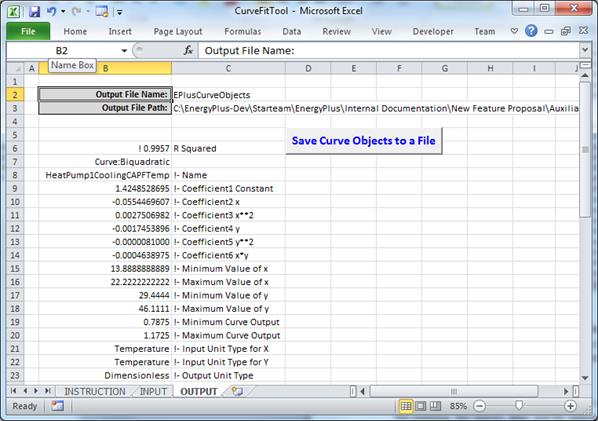
\includegraphics[width=0.9\textwidth, height=0.9\textheight, keepaspectratio=true]{media/image036.jpg}
\caption{Curve Fit Tool Output Interface \protect \label{fig:curve-fit-tool-output-interface}}
\end{figure}

Besides the curve coefficients, the goodness of curve fit indicator statistical parameters \emph{R\(^{2}\)} is also reported. The \emph{R\(^{2}\)} is the ratio of the sum of the squared deviations of the curve fit values from the mean to the sum of the squared deviations of the original data from the mean. R squared values closer to 1.0 are good. The tool has an option to save the curve objects to an output file by running another macro (SaveCurveObjToTextFile). The option output files and the directory path are specified in the OUPUT tab in cells C2 and C3, respectively, as shown in Figure~\ref{fig:curve-fit-tool-output-interface}. If the output file name and path are left blank, then default names, ``EplusCurveObjects.IDF'' and the local directory where the tool is located are used. The local directory where the tool is located must not have write restriction.

Sample EnergyPlus curve objects output file generated using this auxiliary tool.

\begin{lstlisting}

Curve:Biquadratic,
  HeatPumpCoolingCAPFTemp,      !- Name
  1.4248528695,                !- Coefficient1 Constant
  -0.0554469607,                !- Coefficient2 x
  0.0027506982,                !- Coefficient3 x**2
  -0.0017453896,                !- Coefficient4 y
  -0.0000081,                   !- Coefficient5 y**2
  -0.0004638975,                !- Coefficient6 x*y
  13.8888888889,                !- Minimum Value of x
  22.2222222222,                !- Maximum Value of x
  29.4444444444,                !- Minimum Value of y
  46.1111111111,                !- Maximum Value of y
  0.7875,                       !- Minimum Curve Output
  1.1725,                       !- Maximum Curve Output
  Temperature,                  !- Input Unit Type for X
  Temperature,                  !- Input Unit Type for Y
  Dimensionless;                !- Output Unit Type

  Curve:Biquadratic,
  HeatPump1CoolingEIRFTemp,     !- Name
  0.1566419771,                 !- Coefficient1 Constant
  0.0522807347,                 !- Coefficient2 x
  -0.0017986792,                !- Coefficient3 x**2
  0.009523995,                  !- Coefficient4 y
  0.0002405903,                 !- Coefficient5 y**2
  -0.0001781171,                !- Coefficient6 x*y
  13.8888888889,                !- Minimum Value of x
  22.2222222222,                !- Maximum Value of x
  29.4444444444,                !- Minimum Value of y
  46.1111111111,                !- Maximum Value of y
  0.8216,                       !- Minimum Curve Output
  1.3703,                       !- Maximum Curve Output
  Temperature,                  !- Input Unit Type for X
  Temperature,                  !- Input Unit Type for Y
  Dimensionless;                !- Output Unit Type
\end{lstlisting}
